% !TEX root = ../../thesis.tex

\section{Introduction}

As already established earlier on, the Script Assembler introduces a custom syntax added on top of the Robot Framework. It uses annotations such as \texttt{@VERSION} to control the test suit setup. To process this grammar the implementation uses the Lark parsing library~\cite{LarkGithub}. However while the chosen indentation-based syntax is very intuitive for the developers, it introduces technical difficulties for the parser.

Indentation-based scoping is context-sensitive. To find out if a line belongs to a block, the parser needs to know the indentation level of the previous annotation. That requires it that the current indentation depth is saved. While the Lark library provides its own indenter utility for parsing whitespace-scoped languages, it processes indentation globally~\cite{LarkDocsIndent}.
Because the Script Assembler has to differentate between its own language and the contained Robot Framework code, Lark's indenter would generate tokens for Robot Framework code indents which might lead to blocks that close too early.


That is why an additional preprocessing step is required before the Lark parser can evaluate the script. This step is handled by a preprocessor, whose goal is to isolate the meta-language indentation from the content-language indentation before parsing the script.


\section{Design and Transformation Rules}

\subsection{Content vs. Meta-Language Conflict}

The fundamental problem is that both languages use spaces and indentation to define logic and structure. In the Robot Framework, spaces and tabs separate keywords from arguments, and indentation marks the contents of blocks like \texttt{FOR} loops and \texttt{IF} statements, as shown with green highlights in Figure~\ref{fig:indents_highlights}.

At the same time, the Script Assembler uses indentation to determine which lines belong to a specific modifier, as shown with orange highlights in Figure~\ref{fig:indents_highlights}. This leads to the problem of having to somehow seperate those two kind of indents and thus the need for our own Preprocessor instead of the Lark Indenter.

\begin{figure}[h]
    \centering
    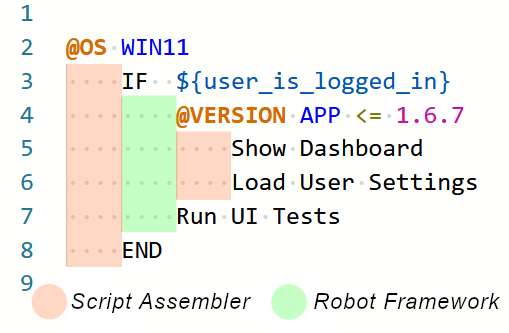
\includegraphics[width=0.75\textwidth]{pics/IndentsHighlights.png}
    \caption{Difference between meta-language and content-language indents. }
    \label{fig:indents_highlights}
\end{figure}

\subsection{Explicit Block Scoping}


To make the syntax context-free, the implicit visual scoping provided by indentation must be changed to explicit block scoping. Clear start and end markers must be defined. This is comparable to the use of curly braces \texttt{\{\}} in C\# or Java, or to opening and closing tags like \texttt{<div>} and \texttt{</div>} in HTML.


For each modifier found by the Preprocessor, the start of the block is simply the modifier itself. The end of the block, shown by a decrease in indentation in the raw script. The Preprocessor marks this by inserting the keyword \texttt{@END}.


With these clear boundaries, the EBNF grammar in Lark is simplified. It only needs to search for the \texttt{@END} token to recognize the end of a block, allowing it to completely ignore the surrounding whitespace.


\subsection{Preserving Indents}


The following example uses several annotations nested within standard Robot Framework control structures. Listing~\ref{lst:raw_script} shows a typical raw Preprocessor input script written by a test developer.


\begin{lstlisting}[caption={Raw input script with nested modifiers}, label={lst:raw_script}, float=htbp]
Setup Test Environment
    @VERSION BIOS == 1.6.1
        Log    Checking BIOS Version
        @OS WIN11
            Install Driver    audio_win11.sys
        Restart Node
\end{lstlisting}


In Listing~\ref{lst:raw_script}, a Robot Framework keyword (\texttt{Setup Test Environment}) is the root scope. Within these block, the outer Script Assembler layer performs a BIOS version check. This block contains a normal Robot command (\texttt{Log}) followed by an inner modifier that checks the operating system. This inner modifier contains a command for a driver installation. Finally, a \texttt{Restart Node} command is executed within the BIOS block, but outside the inner operating system check.


The Preprocessor should calculate the active layers of modifiers and remove only the leading indents belonging to these specific layers. Listing~\ref{lst:preprocessed_script} shows the expected output.


\begin{lstlisting}[caption={Expected Preprocesssor output}, label={lst:preprocessed_script}, float=htbp]

Setup Test Environment
@VERSION BIOS == 1.6.1
    Log    Checking BIOS Version
@OS WIN11
    Install Driver    audio_win11.sys
@END
    Restart Node
@END

\end{lstlisting}


Comparing the two listings shows perfectly how the Preprocessor is supposed to work. The modifier lines themselves (lines 2 and 4 in Listing~\ref{lst:preprocessed_script}) are completely stripped of their indentation. This is needed since the EBNF grammar only sees modifiers that begin with an \texttt{@} symbol, so if it is padded with tabs it is not recognized.

Additionally and most importantly the indentations of the contained language are preserved while the modifier indents are not. For example in the raw text the line \texttt{Install Driver    audio\_win11.sys} was indented three times. Once for the BIOS version check modifier, once for the OS check modifier and once for the actual Robot Framework block. In the result the two modifier indents are removed, leaving only the Robot Framework one.
\texttt{Restart Node}

Finally, the decrease of indentation before the \texttt{Restart Node} command triggers the Preprocessor to insert the \texttt{@END} tag and the open end adds another one lines 6 and 8 in Listing~\ref{lst:preprocessed_script}).


\section{Evolution of the Algorithm}


Developing an appropriate algorithm for this was a technical challenge. The algorithm has to correctly identify mixed indentation levels and clearly distinguish between a line that defines a new lexical scope and a line that just belongs to an existing scope. Parsing context-sensitive, whitespace-dependent meta-languages is a highly complex process, as demonstrated by the evolution of the Preprocessor logic.


\subsection{Linear Depth Counting Approach}


The first version of the Preprocessor used a simple linear mechanism for counting layers. The basic idea was that the depth of a modifier block directly correlated to a simple integer counter. 


In this naive approach, the algorithm maintained a single integer variable called \texttt{current\_layer}, starting at zero. The Preprocessor iterated through the script line-by-line, searching for the \texttt{@} symbol. When it found a modifier, it incremented the \texttt{current\_layer} counter by one. For all following lines, the algorithm removed a number of leading indents exactly equal to the value of \texttt{current\_layer}.


To find the end of a block, the algorithm compared the total number of indents on the current line against the \texttt{current\_layer} variable. If a line had fewer indentations than the active layer count the algorithm assumed that the block had ended. It then inserted an \texttt{@END} tag and decremented the counter. This logic worked in simple situations. However, it contained a fundamental flaw regarding relative and absolute indentation depths.


\subsection{Collision with the Structure of the Content}


The linear depth counting approach unfortunately failed when Script Assembler annotations were mixed with Robot Framework commands that use indents inside a modifier. At that point the absolute count of tabs of a line is no longer just determined by the Script Assembler modifier depth.

Listing~\ref{lst:problem_script} demonstrates the specific edge case that exposed the flaw in the naive algorithm.


\begin{lstlisting}[caption={Problematic edge case}, label={lst:problem_script}, float=htbp]
@VERSION BIOS == 1.2.3
    FOR    ${item}    IN    @{ITEMS}
        @VERSION KBDRIVER != 0.2.5
            Add Item To Cart    ${item}
        Sleep    0.5s
    END
\end{lstlisting}


When verifying the algorithm with Listing~\ref{lst:problem_script}, the error occurs in line 5.

\begin{enumerate}

    \item \textbf{First Modifier:} On line 1, the first \texttt{@VERSION} modifier sets the \texttt{current\_layer} to 1.

    \item \textbf{Inner Modifier:} On line 3, the inner \texttt{@VERSION} modifier increments the \texttt{current\_layer} to 2.

    \item \textbf{Conflicting Line:} On line 5, the \texttt{Sleep} command has exactly 2 leading tabs (one from the outer modifier, and one from the \texttt{FOR} loop).

\end{enumerate}

The algorithm compares the \texttt{Sleep} line's tab count (2) to the \texttt{current\_layer} (2). Since the numbers are equal, the algorithm assumes that the \texttt{Sleep} command is still in the inner \texttt{@VERSION} block. But this is wrong, since the inner \texttt{@VERSION} block started with two tabs, thus requiring any code inside of it to have 3 tabs. This means that the \texttt{Sleep} command actually exits the inner block.

That is why the algorithm unfortunately fails, as seen in Listing~\ref{lst:problem_script_output}. It is counting tabs in \texttt{current\_layer} integer for the indentation and completely ignores how many of these tabs were actually introduced by the contained language.

\begin{lstlisting}[caption={Wrong output of the problematic script with the first approach}, label={lst:problem_script_output}, float=htbp]
@VERSION BIOS == 1.2.3
FOR    ${item}    IN    @{ITEMS}
@VERSION KBDRIVER != 0.2.5
    Add Item To Cart    ${item}
Sleep    0.5s
@END
END
@END
\end{lstlisting}

\subsection{Stack-Based Approach}


To fix this collision, the algorithm required a different approach. Instead of tracking a simple depth integer, it had to explicitly store the absolute indentation level at the exact moment each modifier scope was opened. 

The revised Preprocessor uses a stack to keep track of the indents. Whenever the Preprocessor finds a new modifier, it calculates the exact number of leading tabs on that line and pushes this absolute tab count onto the top of the stack.


This approach maps the nested structure of the text to a linear state history. The value at the top of the stack is always the baseline tab count of the currently active innermost modifier.


Re-evaluating Listing~\ref{lst:problem_script} using this stack-based approach yields the correct behavior:

\begin{itemize}

    \item \textbf{Line 1:} Outer modifier has 0 tabs. Stack becomes: \texttt{[0]}.

    \item \textbf{Line 3:} Inner modifier has 2 tabs. Stack becomes: \texttt{[0, 2]}.

    \item \textbf{Line 4:} Content has 3 tabs. The value 3 is greater than 2 (top of stack). The content belongs to the inner block.

    \item \textbf{Line 5:} The \texttt{Sleep} command has 2 tabs. The value 2 is less than or equal to 2 (top of stack). 

\end{itemize}

\begin{lstlisting}[caption={Correct output of the problematic script with the final approach}, label={lst:problem_script_correct}, float=htbp]
@VERSION BIOS == 1.2.3
FOR    ${item}    IN    @{ITEMS}
@VERSION KBDRIVER != 0.2.5
    Add Item To Cart    ${item}
@END
    Sleep    0.5s
END
@END
\end{lstlisting}

When the algorithm processes line 5, it sees that the current tab count (2) is less than or equal to the top of the stack (2). This triggers the scope resolution logic. The Preprocessor removes the top value from the stack and correctly inserts the \texttt{@END} tag to terminate the inner \texttt{@VERSION} block. Finally, it reaches the end of the file, and since it still has one modifier to close, it ends the output with a final \texttt{@END}.

By using a stack, the Preprocessor can perfectly keep track of at which level a modifier starts and  also where it should end. This makes it entirely unaffected of whatever indentation structures the content uses.

\section{Implementation Details}


The theoretical concepts and the stack-based state machine were implemented in Python. The resulting \texttt{Preprocessor} class encapsulates the state variables, the regular expressions for token identification, and the transpilation loop that processes the script line-by-line. 


\subsection{Initialization and Utilities}


The Preprocessor is initialized with specific regular expressions. These expressions identify valid modifiers and are passed to the Preprocessor by the Parser, removing the need to maintain them in two places. Furthermore, the class defines utility functions to manage the indentations.
Listing~\ref{lst:impl_utils} shows this class initialization alongside these core utility functions.


\begin{lstlisting}[language=Python, caption={Class initialization and indentation utility functions}, label={lst:impl_utils}, float=htbp]
import re
from broker.managers.case.script_assembler.parser_exception import ParserSyntaxError
from logging import Logger

log: Logger = Logger("SCRIPT ASSEMBLER")

class Preprocessor:
    modifier_regex: str
    option_regex: str
    indent_regex: str = r"^(?:\t| {4})+"

    def __init__(self, modifier_regex: str, option_regex: str) -> None:
        self.modifier_regex = modifier_regex
        self.option_regex = option_regex

    def count_indents(self, line: str) -> int:
        """Counts the number of indents at the start of a line."""
        
        match = re.match(self.indent_regex, line)
        if not match:
            return 0
            
        indent_str = match.group()        

        # Count number of indents
        tabs: int = indent_str.count('\t')
        spaces: int = indent_str.count('    ')

        return tabs + spaces

    def remove_indents(self, line: str, amount: int) -> str:
        """Removes 'amount' indents from the beginning of a line."""
        
        match = re.match(self.indent_regex, line)
        if not match:
            return line  # No indents to remove
            
        indent_str = match.group()
        indents = re.findall(r"\t| {4}", indent_str)

        # Remove x indents
        remaining_indents = ''.join(indents[amount:])
        rest_of_line = line[len(indent_str):]

        return remaining_indents + rest_of_line

\end{lstlisting} 


An important detail in Listing~\ref{lst:impl_utils} is the definition of \texttt{indent\_regex}. Different code editors and \glspl{ide} format files differently. The regular expression \verb!r"^(?:\t| {4})+"! handles this reliably. It matches any continuous sequence of leading whitespace. It strictly treats either a single tab character or exactly four spaces as one logical unit of indentation.

This regular expression is then used by two utility functions. First, the \texttt{count\_indents} method calculates the indentation depth of a line. It sums the \texttt{\textbackslash t} characters and blocks of four spaces. This process reduces the visual indentation into a single integer.

Second, the \texttt{remove\_indents} method removes the tabs of the meta-language while preserving the tabs of the content. It stores all indentations into an array. After that, it removes the first elements based on the \texttt{amount} parameter. This parameter corresponds to the current depth of the modifier stack. Finally, it restores the line by puts back together the remaining indents with the actual code.


\subsection{Main Processing Loop}


The \texttt{preprocess} method handles the line-by-line transformation. Listing~\ref{lst:impl_loop} shows the initialization of the state tracking variables: the \texttt{result} string buffer, the \texttt{layer\_tabs} stack, and the \texttt{is\_modifier\_empty} flag.


\begin{lstlisting}[language=Python, caption={Initialization of the main preprocessing loop}, label={lst:impl_loop}, float=htbp, firstnumber=46]

    def preprocess(self, script: str) -> str:

        log.info("Starting preprocessing of robot script...")
        result: str = ""
        layer_tabs: list[int] = []
        is_modifier_empty: bool = False

        for line in script.splitlines():
            stripped: str = line.strip()
            if stripped == "":
                continue
                
            log.debug(f"Processing robot script line: \"{stripped}\"")

            mod: bool = False
            
            if stripped.startswith("@"):
                if stripped == "@END":
                    raise ParserSyntaxError("Cannot have @END in script since it is an internal keyword")
                mod = re.fullmatch(self.modifier_regex, stripped.split(' ')[0][1:]) is not None

            # [...]    

\end{lstlisting}


First, the loop skips any empty lines.
Before using the slower \texttt{re.fullmatch} operation, the algorithm checks is the line starts with an \texttt{@} symbol and thus is a modifier. This filters out the majority of lines. 

If the line begins with that symbol, we check if the modifier is \texttt{@END}. Since this is an internal token only used for terminating the blocks, users are not allowed to use it in raw scripts. That means if it exists in the code, we raise a \texttt{ParserSyntaxError}. This should basically never happen, since the intermediate code is never exposed to the user and \texttt{@END} tags are not highlighted by the later described syntax highlighting (see Chapter~\ref{chap:syntax-highlighting} or Figure~\ref{fig:syntax_highlighting}).

Finally, the algorithm checks if the modifier is valid by matching it against the \texttt{modifier\_regex} passed by the Parser. If it is valid, the \texttt{mod} flag is set to \texttt{True} for later use.

\subsection{Scope Handling}


After reading a line, the Preprocessor decides whether the line belongs to the current scope, opens a new scope, or closes existing scopes. Listing~\ref{lst:impl_stack} illustrates this stack management logic.


\begin{lstlisting}[language=Python, caption={The stack implementation for resolving indentation scopes}, label={lst:impl_stack}, float=htbp, firstnumber=69]

            # [...]
            if len(layer_tabs) > 0:
                tabs: int = layer_tabs[-1]
                cnt: int = self.count_indents(line)

                if mod:
                    line = stripped # don't want any indents on modifier lines

                if cnt <= tabs:
                    while len(layer_tabs) > 0 and cnt <= layer_tabs[-1]:
                        layer_tabs.pop()
                        result += "@END\n"

                        if is_modifier_empty:
                            raise ParserSyntaxError("Cannot have empty modifiers")

                result += self.remove_indents(line, len(layer_tabs)) + "\n"

                if mod:
                    layer_tabs.append(cnt) # adds count of tabs to the stack
                    log.debug(f"Processing modifier; Increasing layer by one")
                is_modifier_empty = False

            else:
                result += f"{line}\n"

            # [...]

\end{lstlisting}


If the stack is not empty, the algorithm compares the absolute indentation count of the current line (\texttt{cnt}) with the top value of the stack (\texttt{tabs}). If the current count is less than or equal to the top value, a scope ends.


This resolution is implemented using a \texttt{while} loop rather than a simple \texttt{if} statement. This ensures proper handling when a single line with fewer indents closes several nested modifier blocks simultaneuosly. For each level removed, the string \texttt{@END\textbackslash n} is appended to the result.


The empty modifier validation occurs inside this loop. If a block is closed but the \texttt{is\_modifier\_empty} flag is still set to \texttt{True} because no inner content was processed, transpilation aborts. This is needed since a modifier without code to modify is pointless. 

That is why the Preprocessor assumes that it is most likely either not correctly indented or a typo by the test developer and needs to raise an \texttt{ParserSyntaxError} to communicate that. Finally, the \texttt{remove\_indents} utility is called to strip the indents of the meta-language before the line is appended to the final output stream.



\subsection{Finalization}


At the end of the loop, new scopes are initialized, and the output is verified before being passed to the Parser, as seen in Listing~\ref{lst:impl_final}.


\begin{lstlisting}[language=Python, caption={Handling the root scope and finalizing the output stream at the end of the file.}, label={lst:impl_final}, float=htbp, firstnumber=97]

            # [...]

            if mod:
                is_modifier_empty = True
                
                if len(layer_tabs) == 0: 

                    # If there aren't any previous modifiers, add initial root layer
                    layer_tabs.append(0)


        # Close any remaining open scopes
        if len(layer_tabs) != 0:
        
            for _ in range(0, len(layer_tabs)):
                result += "@END\n"

        log.info("Finished preprocessing the robot script!")
        
        return result.replace('\r', '')

\end{lstlisting}


If the current line is a modifier and the stack is empty, a root level of \texttt{0} is pushed to the stack to serve as the absolute baseline.

After iterating through the entire file, the algorithm does a final cleanup. If the file ends without returning to zero indentations, the stack still contains unclosed modifier blocks. The logic iterates through all remaining items in the \texttt{layer\_tabs} stack, adding an \texttt{@END} tag for each. Finally, carriage returns are normalized to avoid cross-platform compatibility issues.


\section{Summary}


The Preprocessor acts as a hidden translation layer between the human-readable script and the more machine-centric requirements of the Parser. By using a stack the algorithm properly stores and processes the indentations of the meta-language. It removes the assembler's scoping indicators while retaining the precise indentation required for the Robot Framework runtime environment. Furthermore, the Preprocessor also handles the first validation by rejecting manually added \texttt{@END} keywords and empty modifiers.